\documentclass{article}
\usepackage[utf8]{inputenc}
\usepackage[portuguese]{babel}
\usepackage{array}
\usepackage{booktabs}
\usepackage{upgreek}
\usepackage{listings}
\usepackage{cite}
\usepackage{graphicx}
\usepackage{caption}
\usepackage{url}
% \usepackage{hyperref}
\usepackage{indentfirst}
\usepackage{circuitikz}
\usepackage{empheq}
\usepackage{xcolor}
\usepackage{inconsolata}

\definecolor{codegreen}{rgb}{0,0.6,0}
\definecolor{codegray}{rgb}{0.5,0.5,0.5}
\definecolor{codepurple}{rgb}{0.58,0,0.82}
\definecolor{backcolour}{rgb}{0.95,0.95,0.92}

\lstdefinestyle{mystyle}{
  % backgroundcolor=\color{backcolour},   
  commentstyle=\color{codegreen},
  keywordstyle=\bf,
  numberstyle=\footnotesize\color{codegray},
  % stringstyle=\bf,
  % identifierstyle=\bf,
  basicstyle=\ttfamily,
  breakatwhitespace=false,         
  breaklines=true,                 
  captionpos=b,                    
  keepspaces=true,                 
  numbers=left,                    
  numbersep=5pt,                  
  showspaces=false,                
  showstringspaces=false,
  showtabs=false,                  
  tabsize=2
}

\lstset{style=mystyle}

\begin{document}

\begin{center}
  {\Large\bfseries Equalizador de sons monofônico para celular com circuitos analógicos}\\
\end{center}
\bigskip
\begin{minipage}{.49\textwidth}
  \centering
  Gustavo Soares da Silva Oliveira\\
  n\textordmasculine\ USP: 11261812
\end{minipage}
\begin{minipage}{.49\textwidth}
  \centering
  Natanael Magalhães Cardoso\\
  n\textordmasculine\ USP: 8914122
\end{minipage}
\medbreak
\begin{center}
  Relatório Final - Turma 03\\
  PSI3212: Laboratório de Circuitos Elétricos I\\
  Profa. Dra. Ariana Serrano e Prof. Dr. Roberto Onmori\\
  \bigskip
  22 de Junho de 2020
\end{center}

\renewenvironment{abstract}
{\quotation\small\noindent\rule{\linewidth}{.5pt}\par\smallskip
  {\centering\bfseries\abstractname\par}\medskip}
{\par\noindent\rule{\linewidth}{.5pt}\endquotation}

\begin{abstract}
  Este projeto consiste na construção de um equalizador de sons monofônico para celular com circuitos analógicos. Neste relatório, serão abordadas todas as etapas de construção, ou seja, os fundamentos teóricos, os materiais utilizados, as análises de cada filtro e o circuito final do equalizador. Seguindo as especificações do projeto, a frequência de corte do circuito passa-baixa e passa-alta são 300 e 2200 Hz, respectivamente, e também são as frequências de corte inferior e superior do circuito passa-faixa.
\end{abstract}

\section{Introdução}
Um filtro elétrico tem função de selecionar ou rejeitar uma ou mais faixas de frequência de sinal.

Dentre outras classificações, os filtros possem ser classificados quanto ao aspecto da passagem em passa-baixa, passa-alta ou passa-faixa, quanto aos seus componentes em ativo ou passivo e quanto ao comportamento do sinal em analógico ou digital. \cite{wiki-filtro-eletronico}

Os filtros passivos possuem apenas componentes passivos no circuirto. Eles não requerem um fonte extra (além do sinal), em contraste com os filtros ativos. Na maioria dos casos, os filtros passivos serão compostos apenas de elementos lineares como resistores, capacitores, indutores e transformadores. Filtros passivos mais complexos podem envolver elementos não-lineares, ou elementos lineares mais complexos, como uma linha de transmissão. \cite{wiki-filtro-passivo}

Filtro passa-baixa é o nome dado a um circuito eletrônico que permite a passagem de sinal com frequências abaixo da frequência de corte e atenua o sinal das frequências maiores que a frequência de corte. \cite{wiki-passa-baixa} A figura \ref{fig:teo-passa-baixa} mostra um filtro passa-baixa de primeira ordem, constrído com resistor e capacitor. A frequência de corte pe dada por:

$$
  f_c = \frac{1}{2\pi RC}
$$

\begin{figure}[h!]
  \centering
  \begin{circuitikz}
    \draw 
    (0,0) to[short,o-o] (6,0)
    (0,2) to[R,l_=R,o-] (4,2)
    (4,2) to[short,-o] (6,2)
    (4,0) to[C,l_=C] (4,2)
    (3,0) node[ground]{};
    \draw[draw=none] 
    (0,0) -- (0,2) node[midway] {Entrada}
    (6,0) -- (6,2) node[midway] {Saída};
\end{circuitikz}
  \caption{Circuito passa-baixa.}
  \label{fig:teo-passa-baixa}
\end{figure}

Em contraste com o filtro passa-baixa, o filtro passa-alta passa os sinais com frequência maior que a frequência de corte e atunua os sinais com frequência menor que a frequência de corte. A figura \ref{fig:teo-passa-alta} exibe um filtro passa-alta, também de primeira ordem. \cite{wiki-passa-alta}

\begin{figure}[h!]
  \centering
  \begin{circuitikz}
    \draw 
    (0,0) to[short,o-o] (6,0)
    (0,2) to[C,l_=C,o-] (4,2)
    (4,2) to[short,-o] (6,2)
    (4,0) to[R,l_=R] (4,2)
    (3,0) node[ground]{};
    \draw[draw=none] 
    (0,0) -- (0,2) node[midway] {Entrada}
    (6,0) -- (6,2) node[midway] {Saída};
\end{circuitikz}
  \caption{Circuito passa-alta.}
  \label{fig:teo-passa-alta}
\end{figure}

Já um filtro passa-faixa permite a passagem de sinal com frequência em um certo intervalo e atenua sinais com frequência fora deste intervalo. \cite{wiki-passa-faixa} Na figura \ref{fig:teo-passa-faixa} é possível ver que um filtro passa-faixa é feito de um filtro passa-alta seguido de um filtro passa-baixa. \ref{fig:equalizador}

\begin{figure}[h!]
  \centering
  \begin{circuitikz}
    \draw 
    (0,0) to[short,o-o] (4,0)
    (0,2) to[C,l_=C,o-] (3,2)
    (3,2) to[short,-o] (4,2)
    (3,0) to[R,l_=R] (3,2)
    (2,0) node[ground]{}
    (4,0) to[short,o-o] (8,0)
    (4,2) to[R,l_=R,o-] (7,2)
    (7,2) to[short,-o] (8,2)
    (7,0) to[C,l_=C] (7,2)
    (6,0) node[ground]{};
    \draw[draw=none] 
    (0,0) -- (0,2) node[midway] {Entrada}
    (8,0) -- (8,2) node[midway,xshift=4mm] {Saída};
\end{circuitikz}
  \caption{Circuito passa-faixa.}
  \label{fig:teo-passa-faixa}
\end{figure}

O som é uma onda que viaja em diversos meios de propagação e tem diferentes velocidades em diferentes meios, no ar a sua velocidade é aproximadamente de 343 m/s. O espectro audível para humanos é compreendido na faixa de 20 Hz a 20.000 Hz. Com o intuito de controlar a intensidade do som nas faixas de grave, médio e agudo, vamos montar um equalizador com os resultados dos filtros obtidos no relatório 1, potenciômetros e um amplificador operacional (resultando em um circuito somador). Com isso, analisaremos a resposta em frequência do circuito.

\section{Materiais}
A relação dos componentes usados para montar o circuito equalizador está disposta na tabela \ref{tab:materiais}.

\begin{table}[h!]
  \centering
  \begin{tabular}{ccc}
    \toprule
    Qtd. & Componente      & Especificação \\
    \midrule
    1    & Resistor        & 10 k$\Omega$  \\
    2    & Resistores      & 240 $\Omega$  \\
    2    & Resistores      & 22 k$\Omega$  \\
    3    & Resistores      & 1 M$\Omega$   \\
    1    & Resistor        & 10 k$\Omega$  \\
    3    & Potenciometros  & 200 k$\Omega$ \\
    1    & Potenciometro   & 100 k$\Omega$ \\
    2    & Capacitores     & 2.2 $\upmu$F  \\
    2    & Capacitores     & 3.3 nF        \\
    1    & Amp-op          & LM833D        \\
    1    & Fonte de tensão & 5 $V_pk$      \\
    \bottomrule
  \end{tabular}
  \caption{Componentes utilizados na monstagem do circuito.}
  \label{tab:materiais}
\end{table}

\section{Metodologia}
\subsection{Determinação dos valores de R e C}

Pela equação da frequência de corte
$$
  f_c = \frac{1}{2\pi RC}
$$

Temos que, para um dado valor de $f_c > 0$, o produto $RC$ é dado pela expressão abaixo

$$
  RC = \frac{1}{2\pi f_c}
$$

Considerando que os valores comerciais podem não satisfazer a igualdade acima, podemos definir $\Delta f_c$ como uma função de R e C que calcula a diferença entre o valor teórico do produto RC com o valor comercial.

$$
  \Delta f_c(R, C) = \left\|RC - \frac{1}{2\pi f_c}\right\|
$$

Assim, o valor comercial de $RC$ mais próximo do valor teórico é ocorre quando

$$
  \Delta f_c \rightarrow 0
$$

O algorítmo do Apêndice 1 implementa este cálculo fazendo cerca de 21 mil combinações  de valores de resistência e capacitância em uma tabela de valores comerciais \cite{tabela-comercial} de forma que o valor de $\Delta f_c$ seja mínimo.

\subsection{Montagem do circuito}

O primeiro passo adotado para combinar os filtros individuais foi a adição de um potenciômetro no sinal de saída de cada filtro. Pela lei de Ohm, sabemos que a voltagem é proporcional à resistência ($V = RI$). Assim, o potenciômetro atua como controlador da amplitude do sinal, ou seja, um controlador de volume. A figura \ref{fig:teo-potenciometro} mostra um potenciômetro ligado ao sinal de saída de um circuito passa-baixa. \cite{equalizador}

\begin{figure}[ht!]
  \centering
  \begin{circuitikz}
    \draw 
    (0,0) to[short,o-o] (7.2,0)
    (0,2) to[R,l_=R,o-] (4,2)
    (4,2) to[short] (6,2)
    (4,0) to[C,l_=C] (4,2)
    (6,2) to[potentiometer,name=P,l_=P] (6,0)
    (P.wiper) to[short,-o] (7.2,1)
    (3,0) node[ground]{};
    \draw[draw=none] 
    (0,0) -- (0,2) node[midway] {Entrada}
    (7.2,0) -- (7.2,1) node[midway] {Saída};
\end{circuitikz}
  \caption{Controle de volume com potenciômetro P.}
  \label{fig:teo-potenciometro}
\end{figure}

A fim de sintetizar todos os filtros em um único circuito equalizador utilizaremos um amplificador operacional (amp-op) na configuração somador. O componente amp-op (figura \ref{fig:ampop}) é um circuito analógico integrado (C.I.) e tem como finalidade amplificar tensões que entram nele, gerando um ganho $\upmu$. Em malha aberta, o ganho do amp-op é calculado pela equação $V_{out} = (V_+ - V_-)\upmu$.

\begin{figure}[ht!]
  \centering
  \begin{circuitikz}
    \draw
    (2,2) node[op amp,name=OP,yscale=-1]{}
    ;
\end{circuitikz}
  \caption{Representação de um ampop.}
  \label{fig:ampop}
\end{figure}

A figura \ref{fig:equalizador} mostra o diagrama simplificado do circuito equalizador com os filtros associoados em paralelo e ligados ao polo positivo do amp-op. Além disso, uma resistência R de 1 M$\Omega$ foi colocada em série com a saída de cada filtro com potenciômetro, como na figura \ref{fig:teo-potenciometro}.

\begin{figure}[h!]
  \centering
  \begin{circuitikz}
    \draw
    (6.5,3.75) node[op amp,name=OP,yscale=-1]{}
    (1,5.5) rectangle (3,6.5) node[midway] {Passa-baixa}
    (.5,6.25) -- (.5,4) to[short,*-] (1,4)
    (1,3.5) rectangle (3,4.5) node[midway] {Passa-faixa}
    (.5,4) -- (.5,2) -- (1,2)
    (1,1.5) rectangle (3,2.5) node[midway] {Passa-alta}
    (3,6)++(0,.25) to[short,-o] ++(.2,0) -- ++(.25,0) to[R=R,/tikz/circuitikz/bipoles/length=8mm] ++(1.5,0) -- ++(0,-4)
    (3,6)++(0,-.25) to[short,-o] ++(.2,0) -- ++(.4,0) -- ++(0,-5)
    (3,4)++(0,.25) to[short,-o] ++(.2,0) -- ++(.25,0) to[R=R,/tikz/circuitikz/bipoles/length=8mm] ++(1.5,0) to[short,*-] (OP.+)
    (3,4)++(0,-.25) to[short,-o] ++(.2,0) to[short,-*] ++(.4,0)
    (3,2)++(0,.25) to[short,-o] ++(.2,0) -- ++(.25,0) to[R=R,/tikz/circuitikz/bipoles/length=8mm] ++(1.5,0)
    (3,2)++(0,-.25) to[short,-o] ++(.2,0) to[short,-*] ++(.4,0)
    (OP.-) |- (-.5,.75)
    (OP.out) to[short,o-] ++(.5,0) 
    (OP.out)++(.5,-.75) rectangle ++(2.5,1.5) node[midway] {Auto-falante}
    (-.5,.75) -| ($(OP.out)+(1.75,-.75)$)
    (-.5,.75) node[ground]{} to[sV] ++(0,5.5) -- ++(1.5,0)
    ;
\end{circuitikz}
  \caption{Circuito simplificado do equalizador.}
  \label{fig:equalizador}
\end{figure}

\pagebreak

\section{Resultados e discussão}
\subsection{Análise dos Filtros}

Encontrados os valores de resistência e capacitância que mais se ajustam para cumprir as especificações do projeto, os circuitos passa-baixa e passa-alta foram modelados, como mostra as figuras \ref{fig:circ-baixa} e \ref{fig:circ-alta}.

\begin{figure}[ht!]
  \begin{minipage}{.48\textwidth}
    \centering
    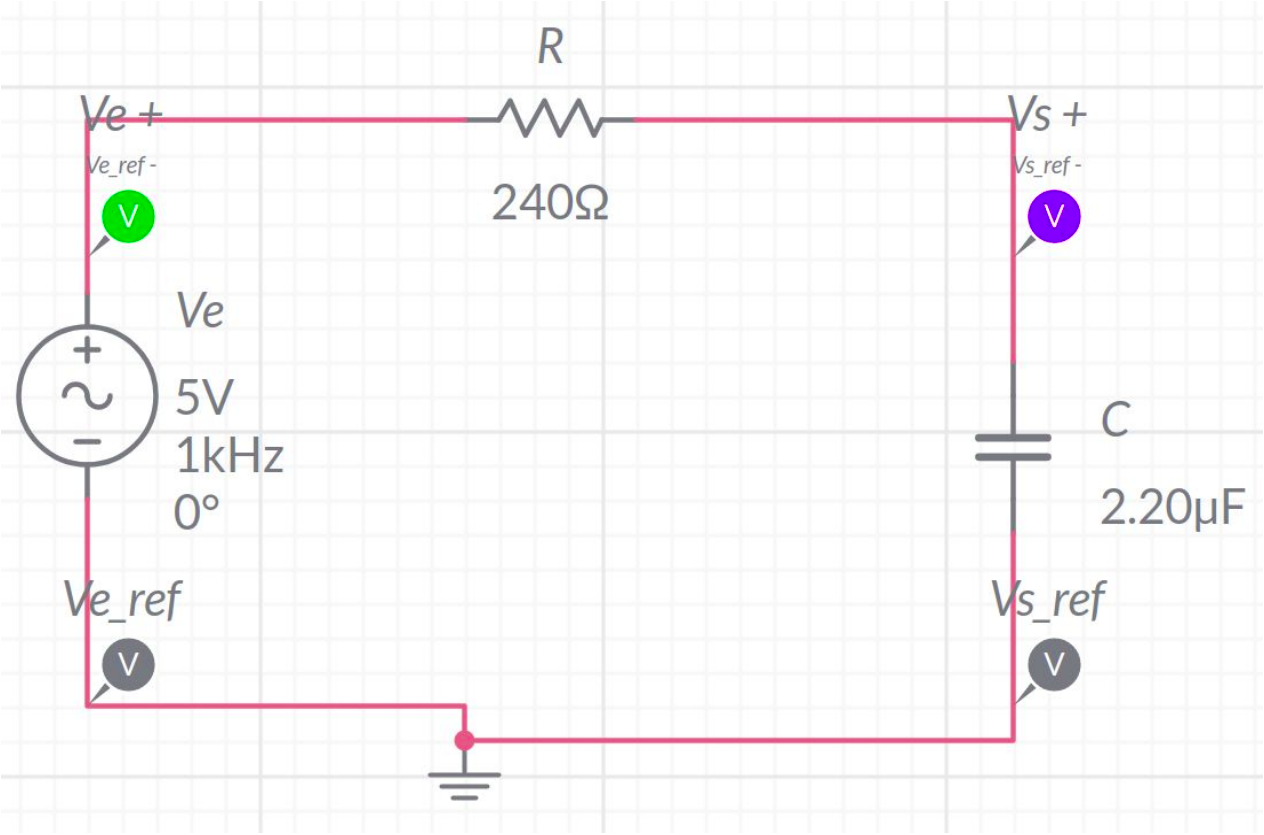
\includegraphics[width=\textwidth]{fig/circ-baixa.png}
    \captionof{figure}{Diagrama do circuito passa-baixa.}
    \label{fig:circ-baixa}
  \end{minipage}%
  \hfill%
  \begin{minipage}{.48\textwidth}
    \centering
    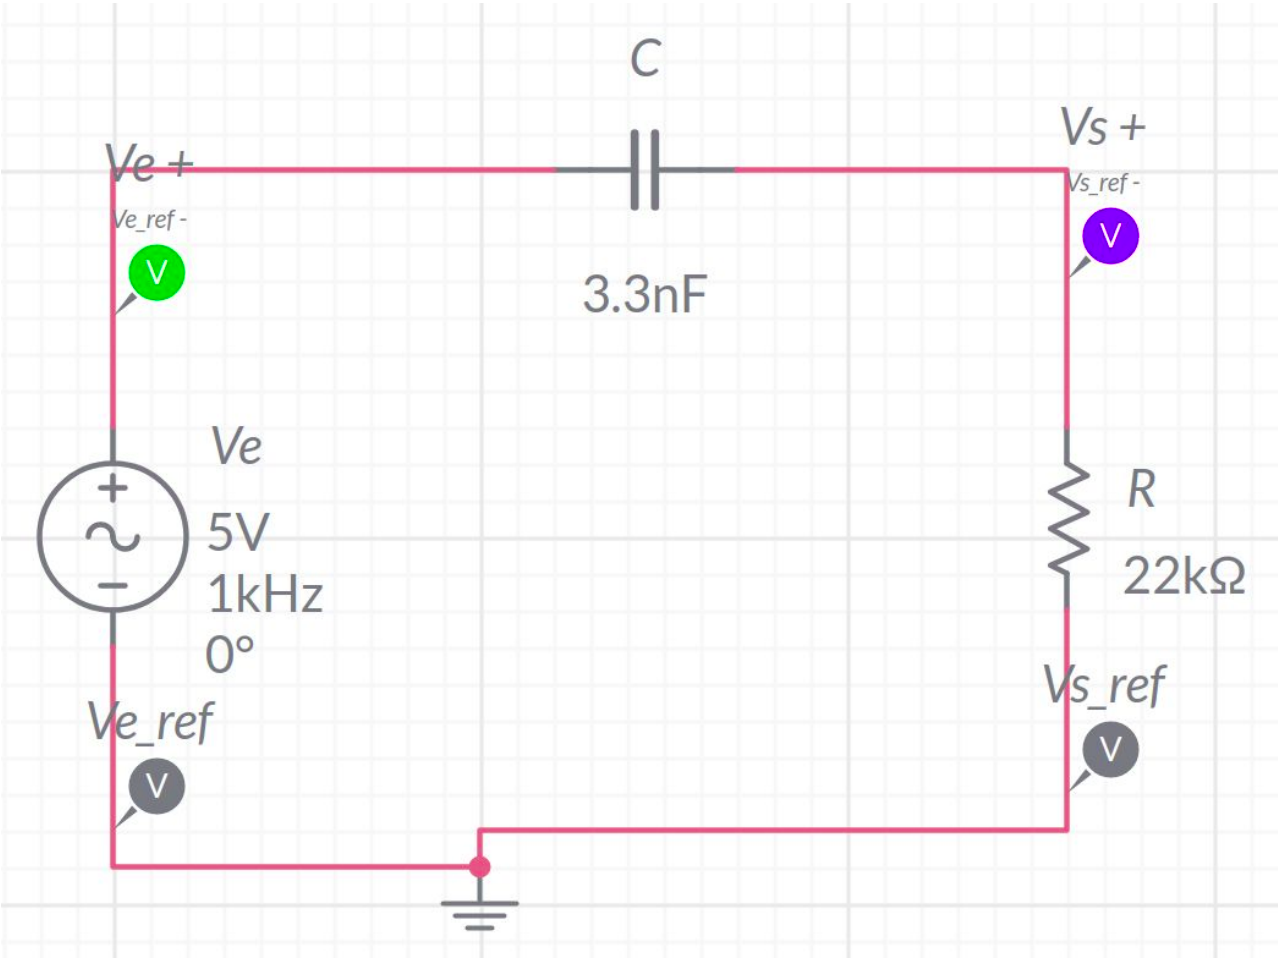
\includegraphics[width=\textwidth]{fig/circ-alta.png}
    \captionof{figure}{Diagrama do circuito passa-alta.}
    \label{fig:circ-alta}
  \end{minipage}
\end{figure}

Assim como especificado na figura \ref{fig:teo-passa-faixa}, o circuito passa-faixa foi modelado usando os valores dos componentes das figuras \ref{fig:circ-baixa} e \ref{fig:circ-alta}.

\begin{figure}[ht!]
  \centering
  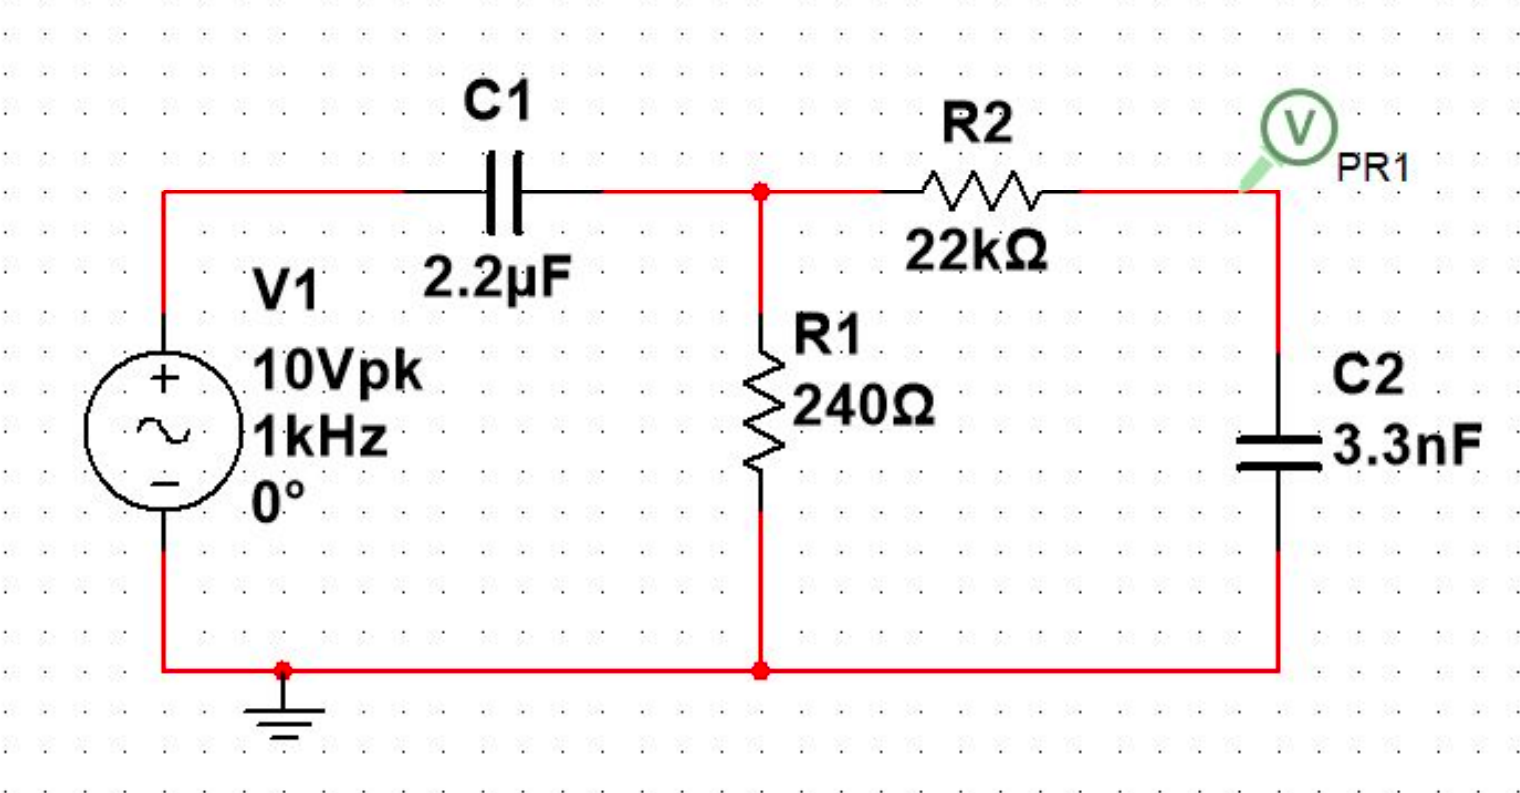
\includegraphics[width=.7\textwidth]{fig/circ-faixa.png}
  \caption{Diagrama do circuito passa-faixa.}
  \label{fig:circ-faixa}
\end{figure}

\pagebreak

A tabela \ref{tab:comb} mostra as melhores combinações de R e C encontradas pelo algoritmo do Apêndice 1 de acordo com os valores de resistência e capacitância da tabela comercial \cite{tabela-comercial}.

\begin{table}[!htbp]
  \centering
  \begin{tabular}{|c|c|c|c|}
    \hline
    \multicolumn{2}{|c|}{Passa-baixa} & \multicolumn{2}{c|}{Passa-alta}                               \\
    \hline
    R                                 & C                               & R            & C            \\
    \hline
    220 $\Omega$                      & 2.4 $\upmu$F                    & 22 $\Omega$  & 3.3 $\upmu$F \\
    240 $\Omega$                      & 2.2 $\upmu$F                    & 33 $\Omega$  & 2.2 $\upmu$F \\
    160 $\Omega$                      & 3.3 nF                          & 22 k$\Omega$ & 3.3 nF       \\
    220 $\Omega$                      & 2.4 nF                          & 33 k$\Omega$ & 2.2 nF       \\
    \hline
  \end{tabular}
  \caption{Algumas combinações de resistência e capacitância.}
  \label{tab:comb}
\end{table}

As figuras \ref{fig:plot-passa-baixa} e \ref{fig:plot-passa-alta} mostram 500 das 21 mil combinações calculadas pelo algoritmo do Apêndice 1. Cada ponto representa uma combinação de R e C. Os melhores candidatos são os pontos mais próximos de zero no eixo das cotas, pois minimizam $\Delta f_c$.

\pagebreak

\begin{figure}[ht!]
  \centering
  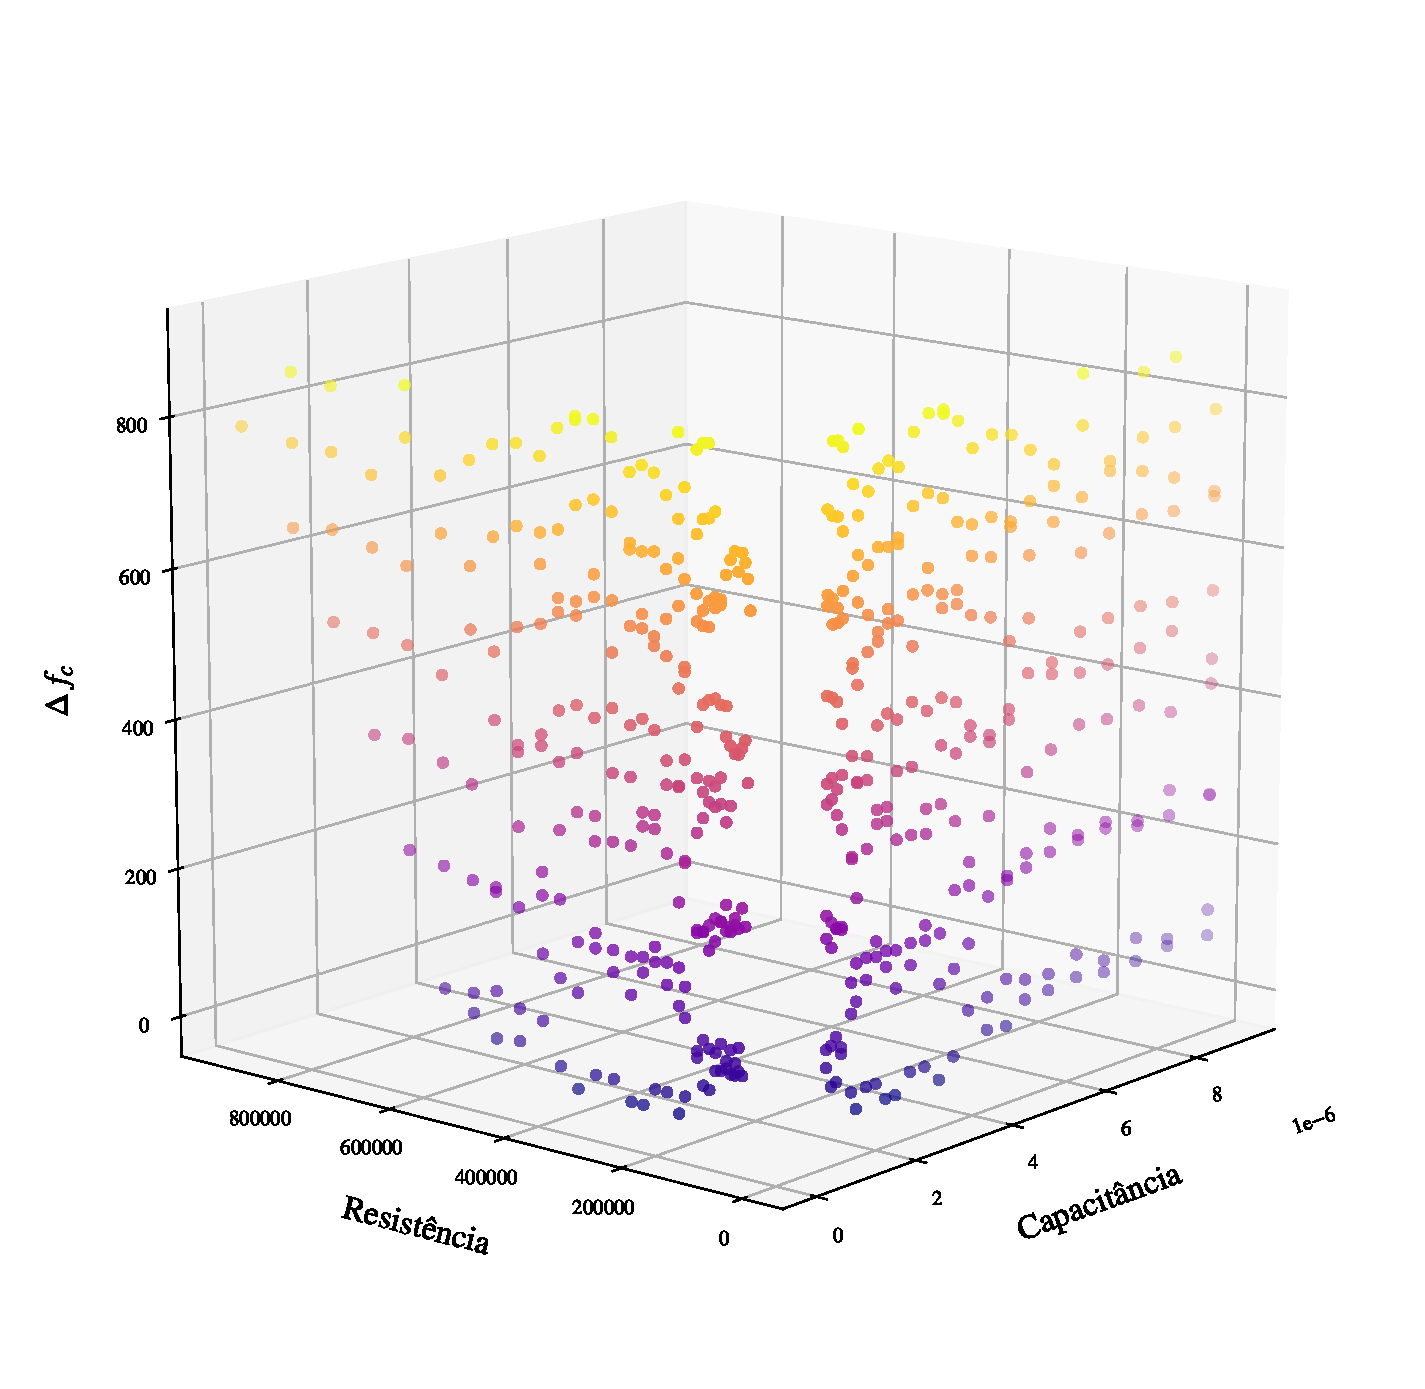
\includegraphics[width=.77\textwidth,trim={7mm 18mm 15mm 34mm},clip]{fig/low.pdf}
  \caption{Gráfico com 500 melhores combinações de R e C que minimizam $\Delta f_c$ para $f_c$ = 300 Hz.}
  \label{fig:plot-passa-baixa}
\end{figure}

\begin{figure}[ht!]
  \centering
  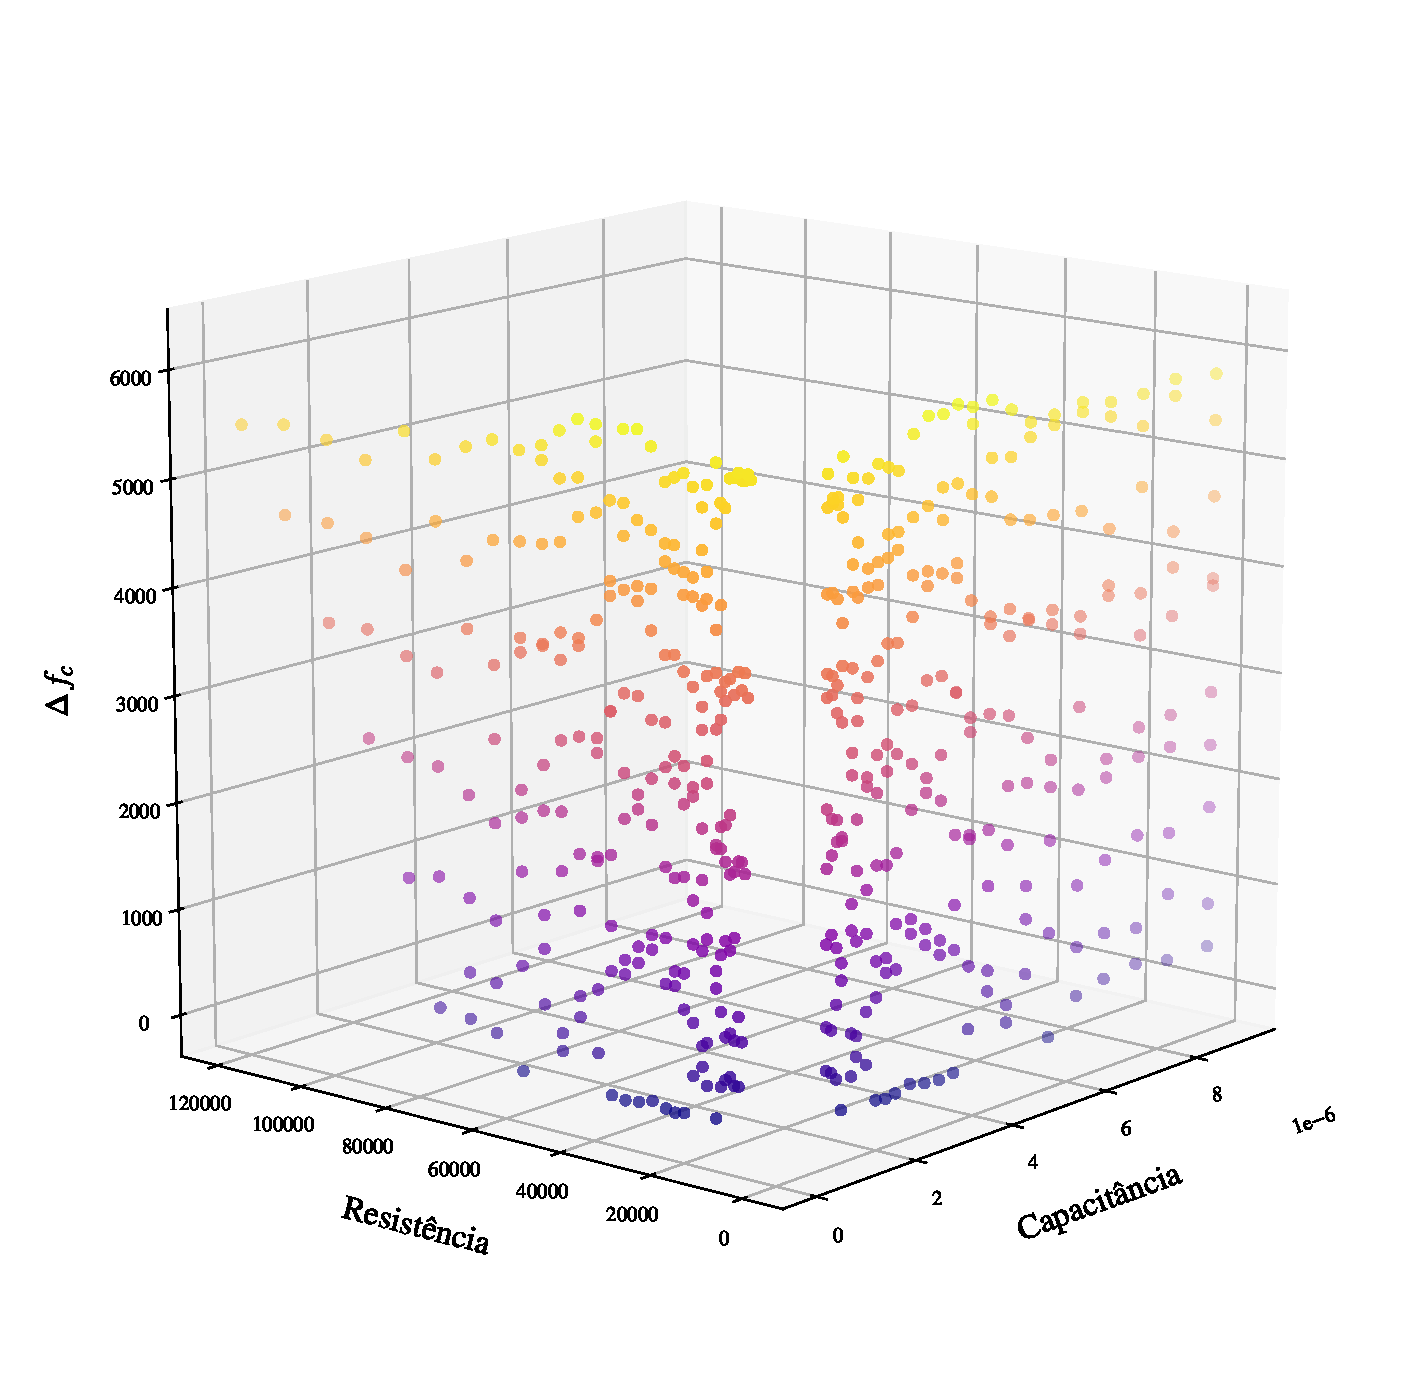
\includegraphics[width=.77\textwidth,trim={7mm 18mm 15mm 34mm},clip]{fig/high.pdf}
  \caption{Gráfico com 500 melhores combinações de R e C que minimizam $\Delta f_c$ para $f_c$ = 2200 Hz.}
  \label{fig:plot-passa-alta}
\end{figure}

Uma forma de inspecionar o comportamento de um circuito sob diferentes frequências é pelo estudo da resposta em frequência. As figuras \ref{fig:ac-sweep-baixa}, \ref{fig:ac-sweep-alta} e \ref{fig:ac-sweep-faixa} mostram os gráficos da fase e ganho em função da frequência para os circuitos passa-baixa e passa-alta.

\begin{figure}[ht!]
  \centering
  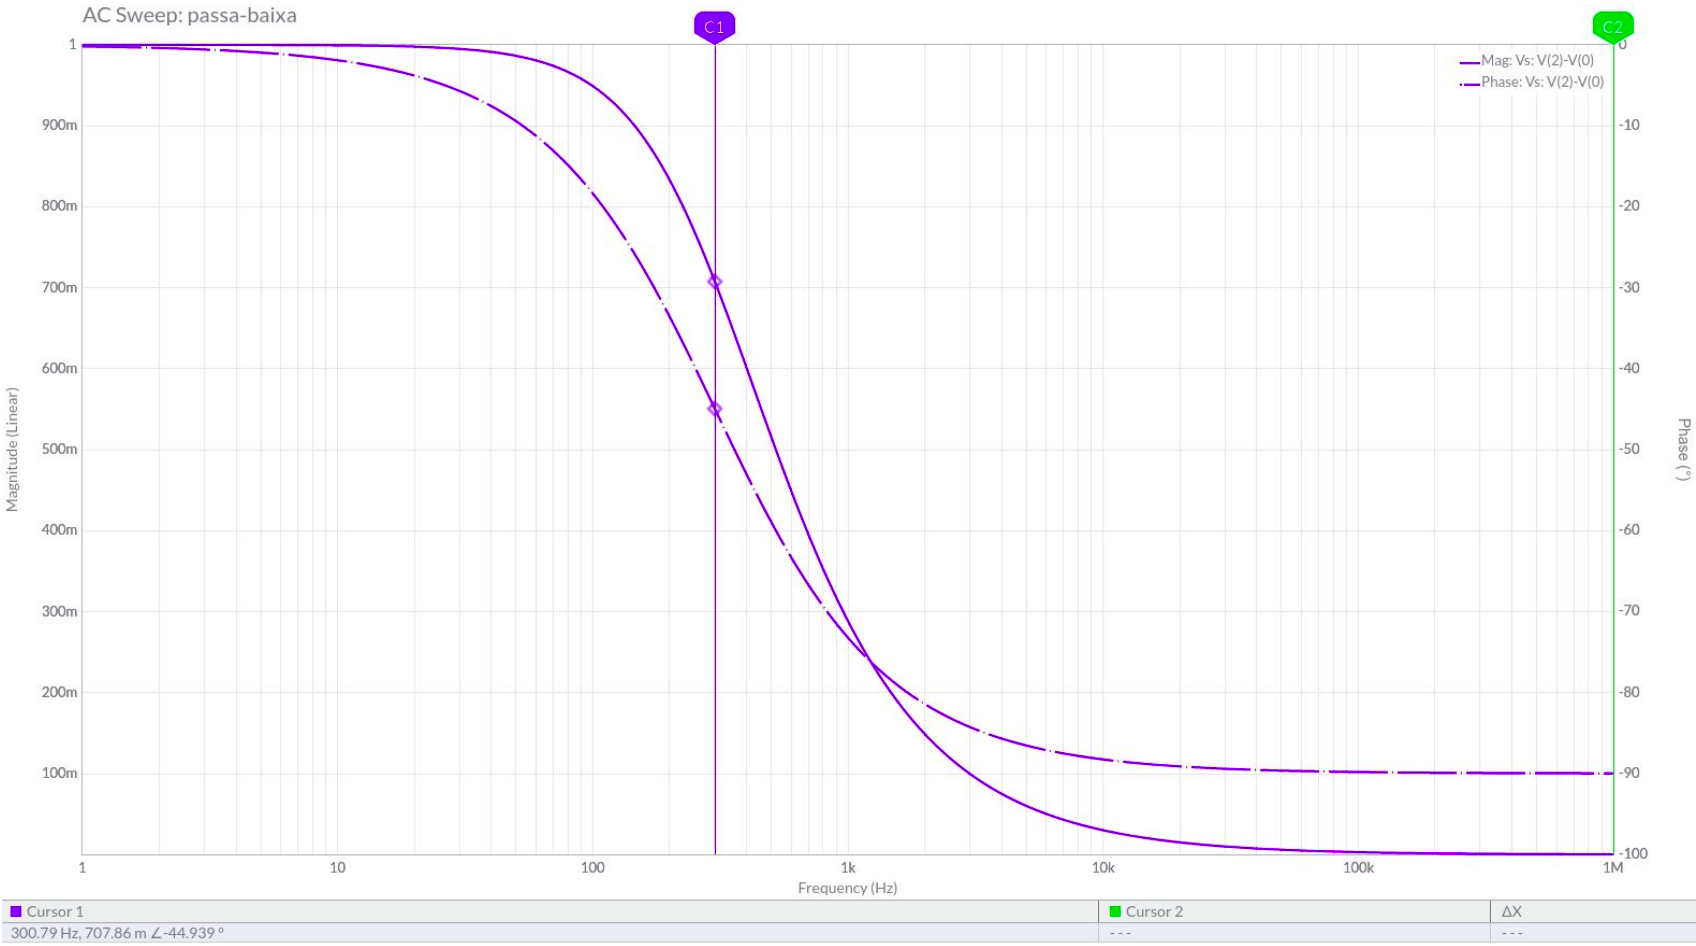
\includegraphics[width=\textwidth]{fig/ac-sweep-baixa.png}
  \caption{Simulação AC Sweep para o filtro passa-baixa. Cursor C1 medindo ganho (magnitude) de 0.708 e fase de -44.939\textdegree\ para uma frequência de 300.79 Hz.}
  \label{fig:ac-sweep-baixa}
\end{figure}

\begin{figure}[ht!]
  \centering
  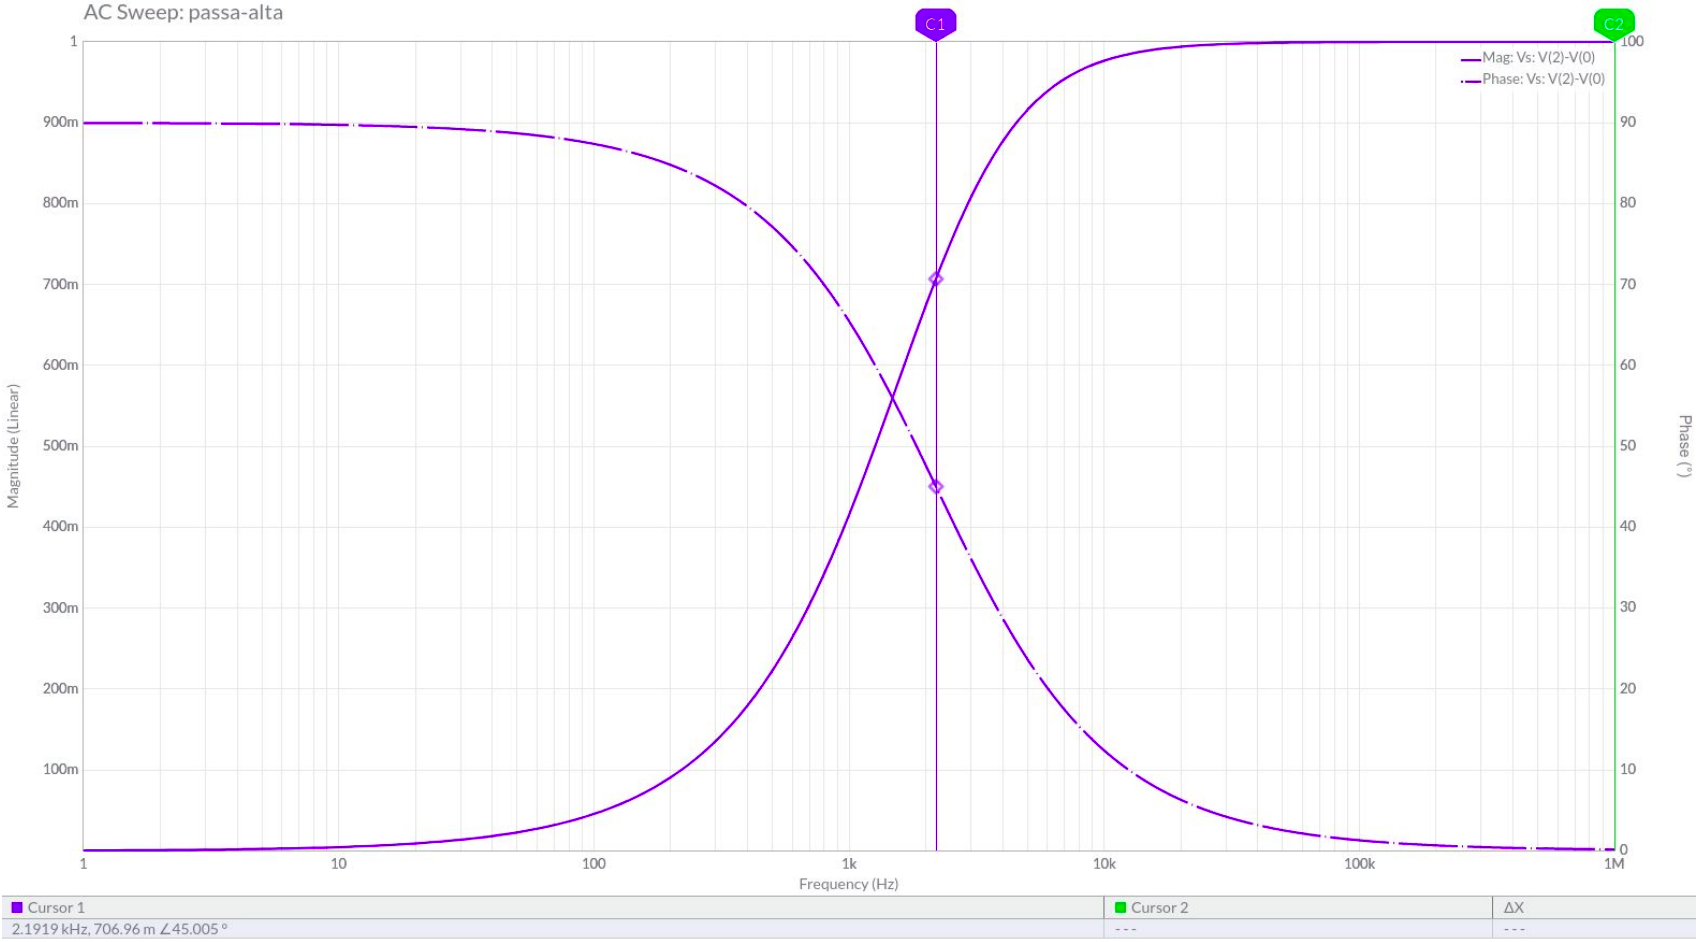
\includegraphics[width=\textwidth]{fig/ac-sweep-alta.png}
  \caption{Simulação AC Sweep para o filtro passa-alta. Cursor C1 medindo ganho (magnitude) de 0.707 e fase -45.005\textdegree\ para uma frequência de 2.192 Hz.}
  \label{fig:ac-sweep-alta}
\end{figure}

\begin{figure}[ht!]
  \centering
  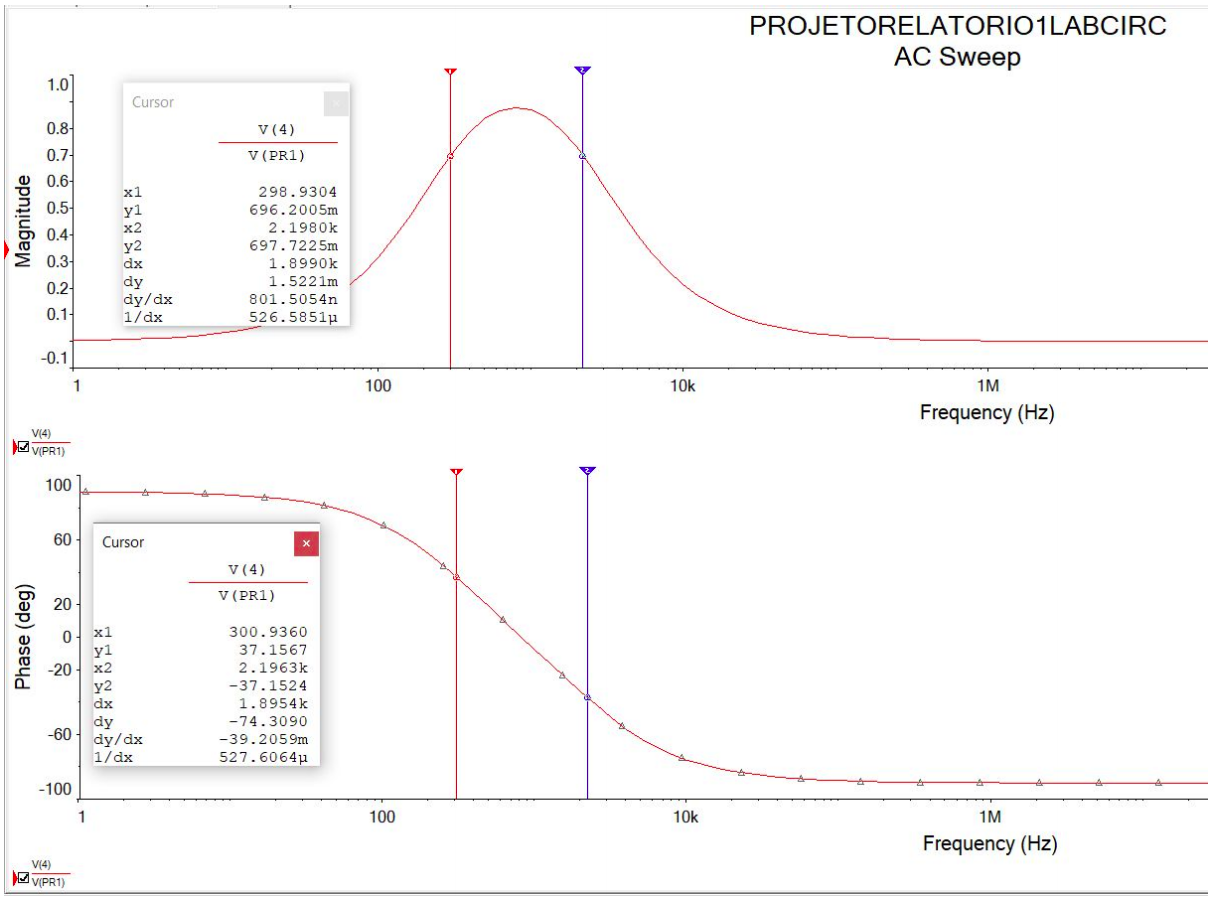
\includegraphics[width=.9\textwidth]{fig/ac-sweep-faixa.png}
  \caption{Simulação AC Sweep para o filtro passa faixa. Os cursores estão medindo as frequências de 300 Hz e 2200 Hz, respectivamente. A magnitude observada foi de 0.696 e 0.697, respectivamente.}
  \label{fig:ac-sweep-faixa}
\end{figure}

\subsection{Análise do circuito final}
\begin{figure}[ht!]
  \centering
  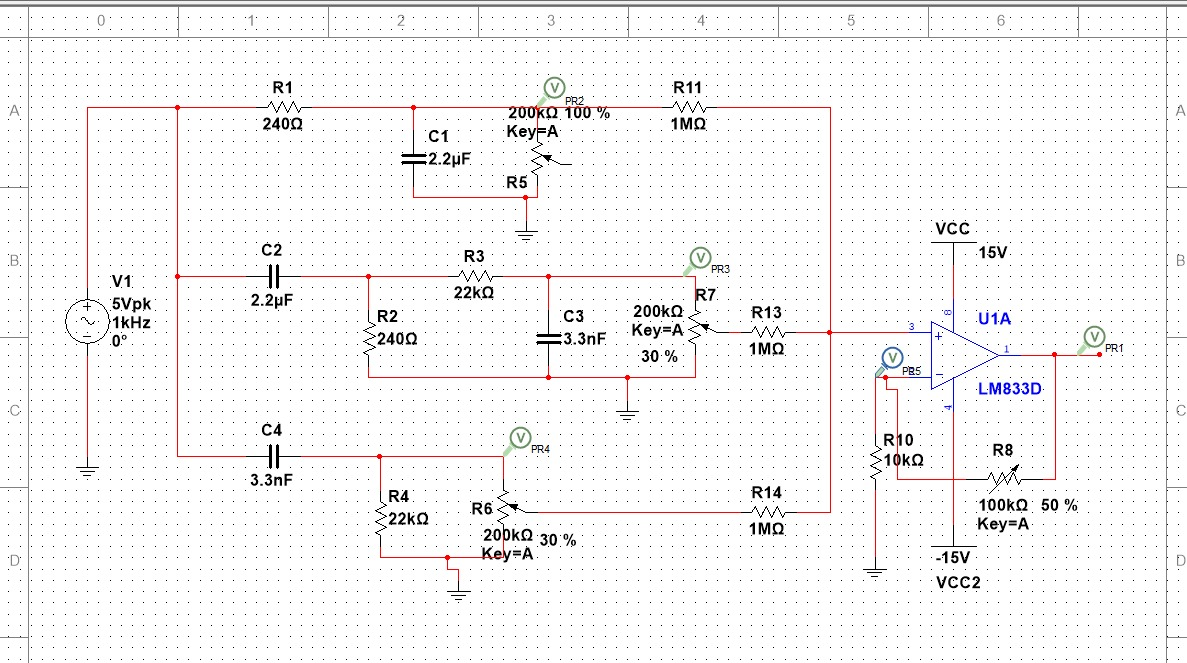
\includegraphics[width=\textwidth,trim={15mm 15mm 15mm 18mm},clip]{fig/circ-equalizador.jpeg}
  \caption{Circuito do equalizador, como descrito na figura \ref{fig:equalizador}, contendo os três filtros das figuras \ref{fig:circ-baixa}, \ref{fig:circ-alta} e \ref{fig:circ-faixa}.}
  \label{fig:circ-equalizador}
\end{figure}

\begin{figure}[ht!]
  \centering
  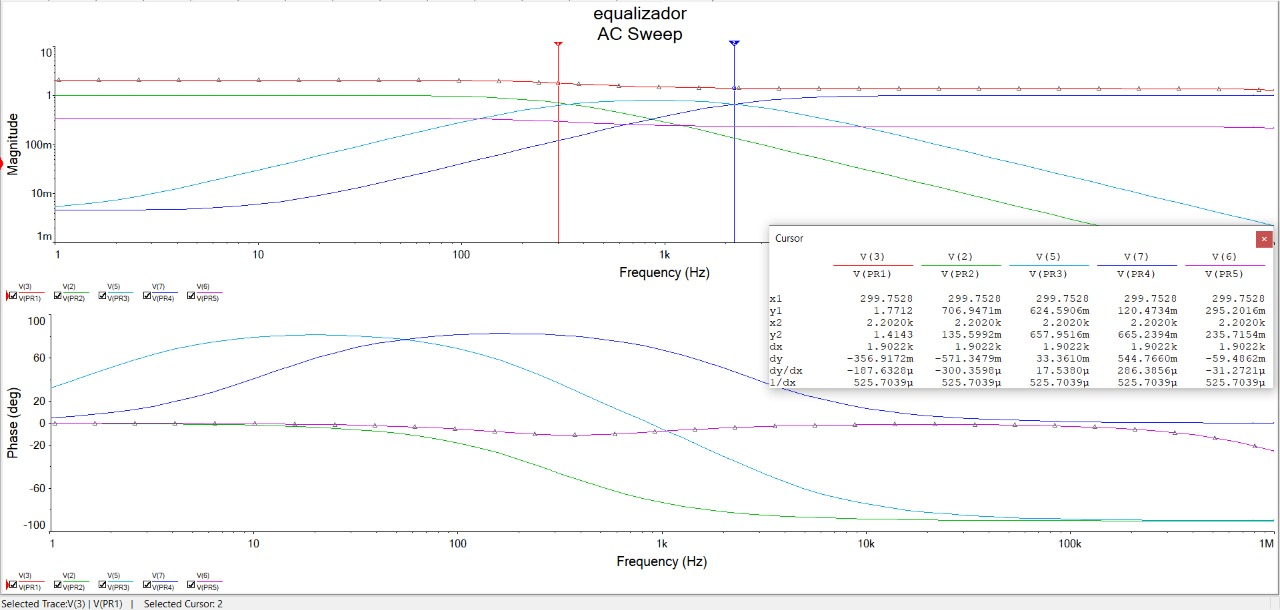
\includegraphics[width=\textwidth]{fig/sim-equalizador.jpeg}
  \caption{Simulação do circuito da figura \ref{fig:circ-equalizador}. O cursor 1 (vermelho) para frequência de 300 Hz e o cursor 2 (azul) para frequência de 2200 Hz.}
  \label{fig:sim-equalizador}
\end{figure}

\begin{figure}[ht!]
  \centering
  \begin{circuitikz}
    \draw
    (5,5) node[op amp,name=OP,yscale=-1]{}
    (OP.-) -| (3,3.5) node[above left]{$V_x$} to[R=$R_2$] ++(0,-2) node[ground]{}
    (OP.+) to[short,-o] ++(-1,0)
    (OP.out) -- ++(.5,0) to[short,i=$i$] ++(0,-1.5) |- (6.7,3.5) to[R=$R_1$] (3,3.5)
    (OP.out) to[short,-o] ++(1.5,0) node[above right]{$V_o$}
    ;
\end{circuitikz}
  \caption{Análise nodal do apm-op.}
  \label{fig:analise-nodal}
\end{figure}

Considerando uma corrente muito baixa alimentando o amp-op, a análise nodal da figura \ref{fig:analise-nodal}, nos dá as seguintes equações:

\begin{empheq}[left=\empheqlbrace]{align}
  &V_o - V_x = R_1 i \label{eq:x1}\\
  &V_x = R_2 i \label{eq:x2}
\end{empheq}

Substituindo \eqref{eq:x2} $\rightarrow$ \eqref{eq:x1}:
\begin{align}
  V_o & = (R_1 + R_2) i \nonumber                            \\
      & = V_x \left(1 + \frac{R_1}{R_2}\right) \label{eq:vo}
\end{align}

Substituindo os valores de $R_1$ e $R_2$ da equação \eqref{eq:vo} pelos valores da figura \ref{fig:circ-equalizador}, obtemos:
\begin{align}
  V_o =  V_x\left(1 + \frac{50 \cdot 10^3}{10 \cdot 10^3}\right) = 6 V_x \label{eq:ganho-teorico}
\end{align}

O ganho é dado por:
\begin{align}
  \upmu = \frac{V_o}{V_x}\label{eq:ganho}
\end{align}

Substiuindo os valores simulados da figura \ref{fig:sim-equalizador} na equação do ganho \eqref{eq:ganho}, temos:
\begin{align}
  \upmu = \frac{1.771}{295.201 \cdot 10^{-3}} \approx 6 \label{ganho-simulado}
\end{align}

Comparando o ganho teórico da equação \eqref{eq:ganho-teorico} com o ganho simulado da equação \eqref{ganho-simulado}, observa-se que os resultados são coerentes.

\section{Conclusão}
Analisando os dados é possível observar a proximidade dos três filtros com o ganho ideal esperado ($1/\sqrt{2} = 0.707$). Já que, o circuito passa-baixa teve magnitude de 0.708, o circuito passa-alta teve magnitude  0.707, e o circuito passa-faixa teve magnitude de 0.696 (em 300 Hz)  e  0.697 (em 2200 Hz).  Com os filtros funcionando conforme o esperado, é configurado o circuito somador de modo que se garantiu o ganho teórico esperado (nesse caso, de 6V). O valor experimental da simulação foi compatível com os cálculos esperados, e mostra que o equalizador está funcionando corretamente.

\bibliography{ref}{}
\bibliographystyle{unsrt}

\newpage

\section*{Apêndice 1}
\begin{lstlisting}[language=Python]
import numpy as np
 
def get_values():
  base = [1.0, 1.1, 1.2, 1.3, 1.5, 1.6, 1.8, 2.0
         2.2, 2.4, 2.7, 3.0, 3.3, 3.6, 3.9, 4.3
         4.7, 5.1, 5.6, 6.2, 6.8, 7.5, 8.2, 9.1]
 
  R, C = [], []
  for p in [0, 1, 2, 3, 4, 5, 6]:
    R += [b * (10 ** p) for b in base]

  for p in [0, -3, -6, -9, -12]:
    C += [b * (10 ** p) for b in base]
    
  return R, C
 
def mesh(R, C, fc):
  f = lambda R, C: np.abs((1 / (R*C)) - (fc*2*np.pi))
    
  mesh = []
  for r in R:
    for c in C:
      mesh.append({'c': c, 'r': r, 'f': f(r, c)})
 
   return sorted(mesh, key=lambda x: x['f'])

R, C = get_values()
low = mesh(R, C, 300)
high = mesh(R, C, 2200)
\end{lstlisting}
\end{document}
